\documentclass{article}
\usepackage{amsfonts}
\usepackage{amsthm}
\usepackage{amssymb}
\usepackage{amsmath}
\usepackage{graphicx}
\usepackage{subcaption}
\usepackage[shortlabels]{enumitem}
\usepackage{xcolor}

\newcommand{\new}[1]{
    \vspace{2mm}
    \noindent
    \textbf{
    \underline{#1}}
}

\def\calO{{\mathcal{O}}}
\def\th{{\theta}}
\def\_{{\hspace{1mm}}}
\def\<{{\langle}}
\def\>{{\rangle}}


\newcounter{problemcnt}
\setcounter{problemcnt}{0}

\newcommand{\Problem}{{
    \vspace{5mm}
    \stepcounter{problemcnt}
    \noindent
    \arabic{problemcnt}. 
}
}

\newcommand{\nProblem}[1]{
    \vspace{5mm}
    \noindent
    \setcounter{problemcnt}{#1}
    \arabic{problemcnt}. 
}


\newcommand{\Proof}{{
    \vspace{2mm}
    \noindent
    \textbf{
    \underline{Proof}}
}
}

\newcommand{\textOr}{
    {
        \hspace{5mm}
        \textrm{or}
        \hspace{5mm}
    }
}

\newcommand{\textAnd}{
    {
        \hspace{5mm}
        \textrm{and}
        \hspace{5mm}
    }
}

\newcommand{\m}{
    \cdot
}

\newcommand{\Pt}[1]{
    $P_{#1}$
}

\newcommand{\Szpt}[1]{
    $|P_{#1}|$
}

\newcommand{\bbinom}[2]{
    \bigg(\binom{#1}{#2}\bigg)
}



\begin{document}
\begin{center}
\LARGE
Combinatorics HW2

\Large
Daniel Son
\end{center}

Section 2.7: 22, 23, 26, 37, 38, 45, 47, 53

Section 3.4: 4, 9, 14, 19 (hint: 19
(c) is asking for a value of mn which need not be minimal. But you should
be able to easily justify that it is valid.)


Additional Problem 1 (Problem 19 (d)). Show that any 4 points within an
equilateral triangle of side length 1 include 2 points which are distance at most
 $1\sqrt{3}$ apart.
Hint.You can show this by covering the shape with 3 regions with diameter1 $1\sqrt{3}$ .
It is ok if these regions overlap.

\new{Sec2.7 q22}
A footrace takes place among four runners. If ties are allowed (even all four 
runners finishing at the same time), how many ways are there for the race to 
finish? 

\new{Solution}
Divide all outcomes of the solutions into four parts:
\begin{itemize}
    \item $P_1$, all players tied
    \item $P_2$, all competitiors were either 1st or 2nd place
    \item $P_3$, all competitiors were either 1st, 2nd, or 3rd place
    \item \Pt{4}, nobody tied
\end{itemize}

It is trvial to count \Szpt{1} and \Szpt{4}. They are 1, and $4! = 24$ respectively. 
To count \Szpt{2}, we allocate each player a number 1 or 2, resembling their 
result in the race. If all 
players are alloted the same number, the arrangement will not be included 
in the part. Count \Szpt{2} by the principle of subtraction:

\[
    |P_2| = 2^4 - 2 = 14
\].

For the third part, we adopt a constructive method. Among the 
four players, choose the player who wins 1st place, 2nd place, and third place. 
The last player can be chosen to be of any standing. We notice that 
each arrangement overcounts by a factor of 2. Call the four runners 
a, b, c, d. The case where a, b wins 1st place, c wins 2nd place, 
and d wins 3rd place can be constructed by choosing 
a, b, c to be 1, 2, 3rd place respectively and letting d to be first place. 
Another possible construction is by letting d, b, c to be 1, 2, 3rd place 
and letting a be first place. For any arrangement, the construction 
overcounts by a factor of 2. Thus, 

\[
    |P_3| = 4\m3\m2\m3 /2 = 36
\]

Add the sizes of all the parts to obtain the answer.

\[
    |P| = \sum_{i\leq 4} |P_i| = 1 + 14 + 36 + 24 = \boxed{75}
\]


\new{Sec2.7 q23}
Bridge is played with four players and an ordinary deck of 52 cards. Each player 
begins with a hand of 13 cards. In how many ways can a bridge game start? 
(Ignore the fact that bridge is played in partnerships.) 

\new{Solution}
The rule of Bridge dictates that all the players must play 
a card of the same suit from the card that is dealt from the first player, 
unless the player does not have any card that is from the same suit. 
Observe that any play of four cards can be justified. Call the players 
who plays after the first player as subsequent players. To justify any 
subsequent players dealing a card that is from the different suit from 
the first card, let the first player to own all the cards from the same 
suit other than the cards that are dealt. 

Proceed by principle of multiplication. 
Let the four players be a, b, c, d. After choosing the first player, 
the order in which the players deal the card is determined. After 
choosing one of the four players, choose the card each player plays. 
The number of all possible openings are
\[
    4\m P(52, 13) = \boxed{15816970575644958720000}
\]

\new{Sec2.7 q26}
A group of mn people are to be arranged into m teams each with n players. 

(a) Determine the number of ways if each team has a different name. 

(b) Determine the number of ways if the teams don't have names. 


\new{Solution}
Question (a) can be answered by the concept of multinomials. Label each 
team as team 1, team 2, ... team m. Assigning each person to a team 
can be converted to assigning $n\m m$ people a number from the 
cannonical set $[m]$ where each number can be used n times. By ordedring 
each person in a fixed order and listing out their team names, we obtain 
a string of $n\m m$ numbers. The number of all possible strings can be counted by

\[
    \binom{n\m m}{n, \dots, n} = \boxed{\frac{(n\m m)!}{(n!)^m}}
\]

To answer question (b), enfoce order by dividing $m!$.

\[
    \boxed{\frac{(n\m m)!}{(n!)^m\m(m!)}}
\]

\new{Sec2.7 q37}
A bakery sells six different kinds of pastry. If the bakery has at least a dozen of 
each kind, how many different options for a dozen of pastries are there? What 
if a box is to contain at least one of each kind of pastry?

\new{Solution}
For there are a dozen of pastries of each kind, it is possible to fill the 
box with one type of pastries. In other words, the restriction of pastries of 
each kind will not cause overcounting. The possible ways of filling the box 
with pastry of any kind can be counted as the number of multisets with 12 
elements formed from six elements. Hence,

\[
    \bbinom{6}{12} = \binom{17}{5} = \boxed{6188}
\]

As for the case where each box is required to include at least 
one pastry of each kind, we apply a constructive method. Include the 
six pastries of different type, and fill the remaining slots. By the 
same logic above, we write the answer.

\[
\bbinom{6}{6} = \binom{11}{5} = \boxed{462}
\]

\new{Sec2.7 q38}
How many solutions are there to the equation
\[
    x_1+x_2+x_3+x_4 = 30
\]
that satisfy $x_1\geq2, x_2\geq0, x_3 \geq-5, x_4 \geq8$?

\new{Solution}
We apply the substitution $a := x_1-2, b:=x_2, c:=x_3 +5, d:=x_4 - 8$. 
The equation is converted to
\[
    a + b + c + d = 25
\]
where $a, b, c, d \in \mathbb{N}$. The number of solutions can 
be computed with the starts and bars method. Consider arranging 
25 stars and three bars. We count the solution to be
\[
    \binom{28}{3} = \boxed{3276}
\]

\new{Sec2.7 q45}
Twenty different books are to be put on five book shelves, each of which holds 
at least twenty books. 

(a) How many different arrangements are there if you only care about the 
number of books on the shelves (and not which book is where)? 

(b) How many different arrangements are there if you care about which books 
are where, but the order of the books on the shelves doesn't matter?

(c) How many different arrangements are there if the order on the shelves does 
matter?


\new{Solution}
Question a) can be dispatched with ease. Consider arranging 20 stars and four bars. 
Or, one can count the number of multisets with size 20 with five distinct elements. 
Either way, the answer is
\[
    \bbinom{5}{20} = \binom{24}{4} = \boxed{10626}
\]

For question b), arrange the books in random order, and assign each 
book into a shelf. By the principle of multiplication we count
\[
    5^{20}= \boxed{95367431640625}
\]

For question c), we use the results from a). Define the shape of a 
book arrangement to be the number of books in each shelf. We purport that 
for each shape, there are $P(20, 20) = 20!$ ways to arrange the books. 
For any permutation of the books, start filling up from the top shelf according 
to the shape. By the principle of multiplication, we count 
\[
    \binom{24}{4} \m 20! = \boxed{25852016738884976640000}
\]

\new{Sec2.7 q53}
Find a bijection between the cannonical set $[n]$ and the towers 
$A_0 \subsetneq A_1 \subsetneq \cdots \subsetneq A_n$ where $|A_i| = i$
for $i \in [n] \cap \{0\}$. 

\new{Solution} 
From the permutation $\{a_1, a_2, \dots, a_n\}$, we construct 
$A_i$ in the following manner. 
\begin{itemize}
    \item $A_0 = \emptyset$
    \item $A_{i+1} = A_i \cup \{i + 1\}$ for $i \in \{0, 1, \dots, n -1\}$
\end{itemize}

Also, from the towers, it is possible to obtain a permutation. It suffices 
to compute the numbers $a_i$ from the towers. Notice that the set 
$A_{i}\setminus A_{i -1}$ has exactly one elements due to the size 
condition. Let this unique element be $a_i$. 

From any permutation, apply the first procedure to obtain a tower of sets. 
Then, apply the second procedure to obtain the same permutation that 
we have started with. Also, applying the second procedure and then the 
first procedure to any random tower of sets results in the same tower of sets. 
Thus, both procedures must describe a bijection between permutation and tower of sets. 
\hfill \qed

\new{Sec3.4 q4}
Show that if n + 1 integers are chosen from the set {1, 2, ... , 2n}, then there are 
always two which differ by 1. 

\new{Solution} Combine the choice of $n+1$ numbers to construct 
set $A$. Define $B:=\{a+1|a\in A\}$. All elements in $A, B$ are 
bounded under by 1 and over by $2n+1$. Thus, the set $A\cap B$ must 
have at most $2n + 1$ elements. If $A$, $B$ are distinct set, that is 
$A \cap B = \emptyset$, it must be
\[
    |A \cup B| = |A|+|B| = 2n + 2
\] .
But this contradicts the fact that $|A\cup B| \leq 2n+1$. 
There must be a common element between $A, B$. Call this element $x$. 
By construction of $B$, there exists an integer $y \in A$ such that $y + 1 = x$. 
The two integers $x, y \in A$ sees witness to the theorem. 
\hfill \qed


\new{Sec3.4 q9}
In a room there are 10 people, none of whom are older than 60 (ages are given in 
whole numbers only) but each of whom is at least 1 year old. Prove that we can 
always find two groups of people (with no common person) the sum of whose 
ages is the same. Can 10 be replaced by a smaller number?

\new{Solution} Consider the choice of any group of 4 or 5 people among 
the whole group. The age of this subgroup will be in range of $[4, 300]$. 
There are a total of $\binom{10}{4} + \binom{10}{5} = 462$ ways to choose such 
groups. Let the pigeons be the choice of any group, and the hole be the 
sum of the ages in a group. $462 > 297$ so there must be two subgroups of 
the same size, where the group is distinct. From the choice of two groups, 
exclude the people who belong to both subgroups to obtain two subgroups that 
have the same cumulative age sum. For example, if the group $\{a, b, c, d, e\}$ and 
group $\{a, b, c, D\}$ have the same cumulative sum, we write
\[
    a + b+ c+d+e = a+b+c+D \textAnd d+e = D
\]
Thus, the two subgroups $\{d, e\}, \{D\}$ have the same age sum. 
Since all people are aged at least one years old, it is impossible to have 
to subgroups $\emptyset$, $\{a\}$. 

Indeed, this logic can be extended to show that the property holds 
for a group of 9 people. Instead of choosing a group of four or five 
people, choose all subgroups that include less than 4 people, excluding the 
emptyset. 

\[
    \sum_{i = 1}^{4} \binom{9}{i} = 255 > 236
\]

By the same argument above, two subgroups with the same cumulative age sum 
must exist. 

\hfill \qed

\new{Sec3.4 q14}
A bag contains 100 apples, 100 bananas, 100 oranges, and 100 pears. If I pick 
one piece of fruit out of the bag every minute, how long will it be before I am 
assured of having picked at least a dozen pieces of fruit of the same kind?

\new{Solution}
Apply the strong form of the pigeonhole principle. Let each type of 
fruit be the holes, and the fruit iteslf pigeons. Given $11\m4+1$ pigeons, 
and four holes, there must exist a hole that has at least $11 + 1 = 12$ 
pigeons. Hence, we must pick 45 fruits which will take 45 minutes.
\hfill \qed

\new{Sec3.4 q19}

(a) Prove that of any five points chosen within an equilateral triangle of side 
length 1, there are two whose distance apart is at most 1/2. 

(b) Prove that of any 10 points chosen within an equilateral triangle of side 
length 1, there are two whose distance apart is at most 1/3. 

(c) Determine an integer mn such that if mn points are chosen within an equilateral triangle of side length 1, there are two whose distance apart is at 
most 1/n. 

\new{Solution}

a) Cut the equilateral triangle into four smaller triangles, as shown 
in figure 1. At least two of the points must fall into the same subtriangle. 
It is known that within a equilateral triangle, the bottom limit of the distance 
between the two triangle is its sidelength. Hence, we guarantee that 
the minimum distance between any two points in the larger triangle must be 
at least 1/2. Figure 1 shows an arrangement of four points that 
satisfy this condition. 
b) Cut the equilateral triangle into nine smaller triangles, as shown 
in figure 2. By the same argument used in a), the minimum distance 
between any two points is greater than 1/3. Figure 2 also shows an arrangement 
that demonstrates this lower bound. 

c) By the same logic above we observe that if
\[
    m_n:= \bigg(\sum_{i \leq n}2n-1\bigg) +1= n^2+1 
\]
Then by the pigeonhole priciple, the lower bound of the distance
 between two points is $1/n$, by the logic used in a). Slice 
 the triangle by $n-1$ horizontal lines, left-tilted lines, 
 right-tilted lines which are all equidistant. This will slice 
 the triangle into $n^2$ smaller equilateral triangles. Figure 3 demonstrates
 such a cutting for $n = 4$. 
 However, 
 note that a set of points that satisfy this upper bound of minimum 
 distance is not guaranteed. 

 \begin{center}
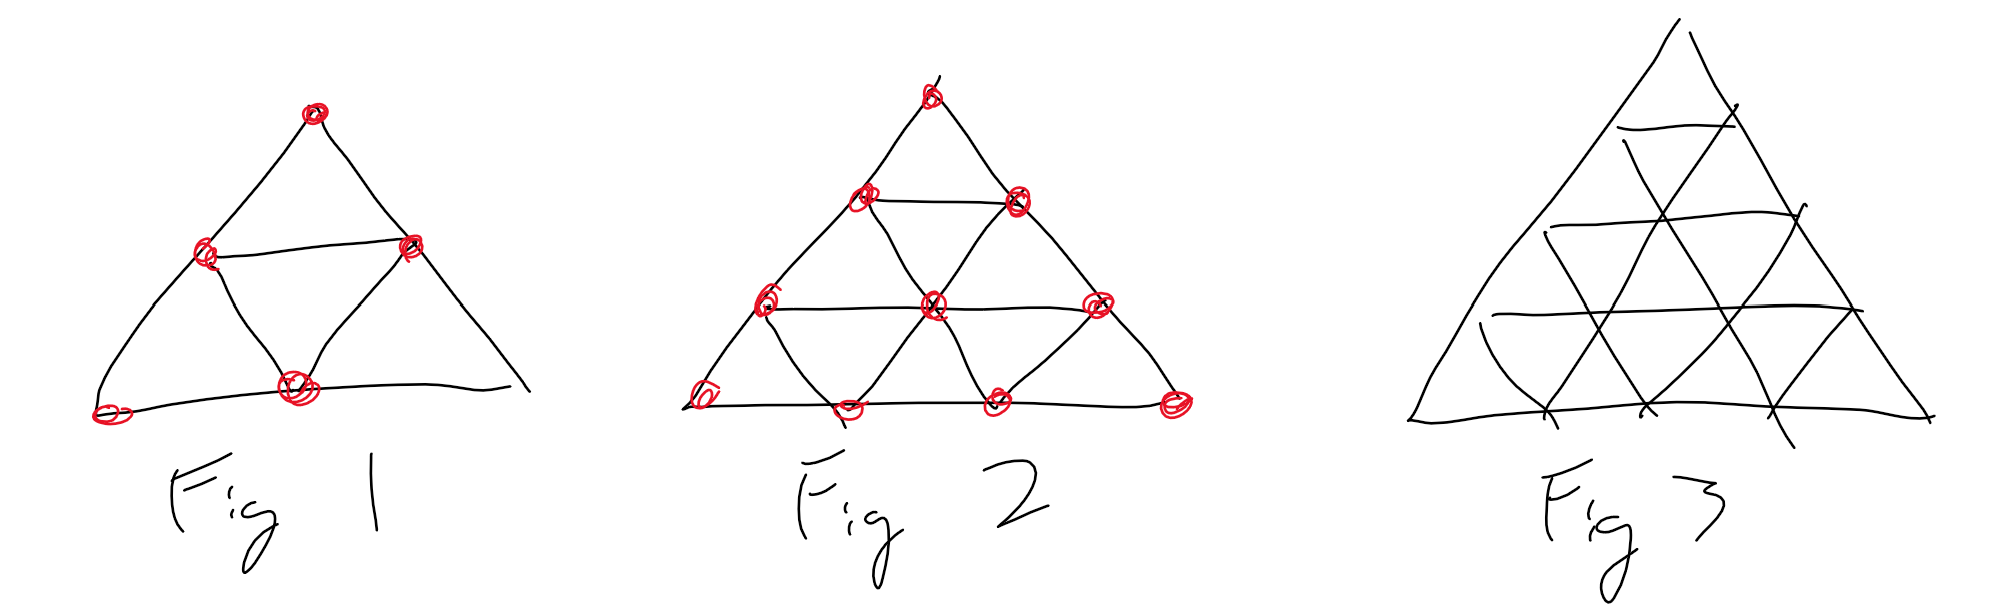
\includegraphics[width = .5\linewidth]{Figures.png}
 \end{center}

 \hfill \qed

 \new{Additional Problem 1}


 \begin{center}
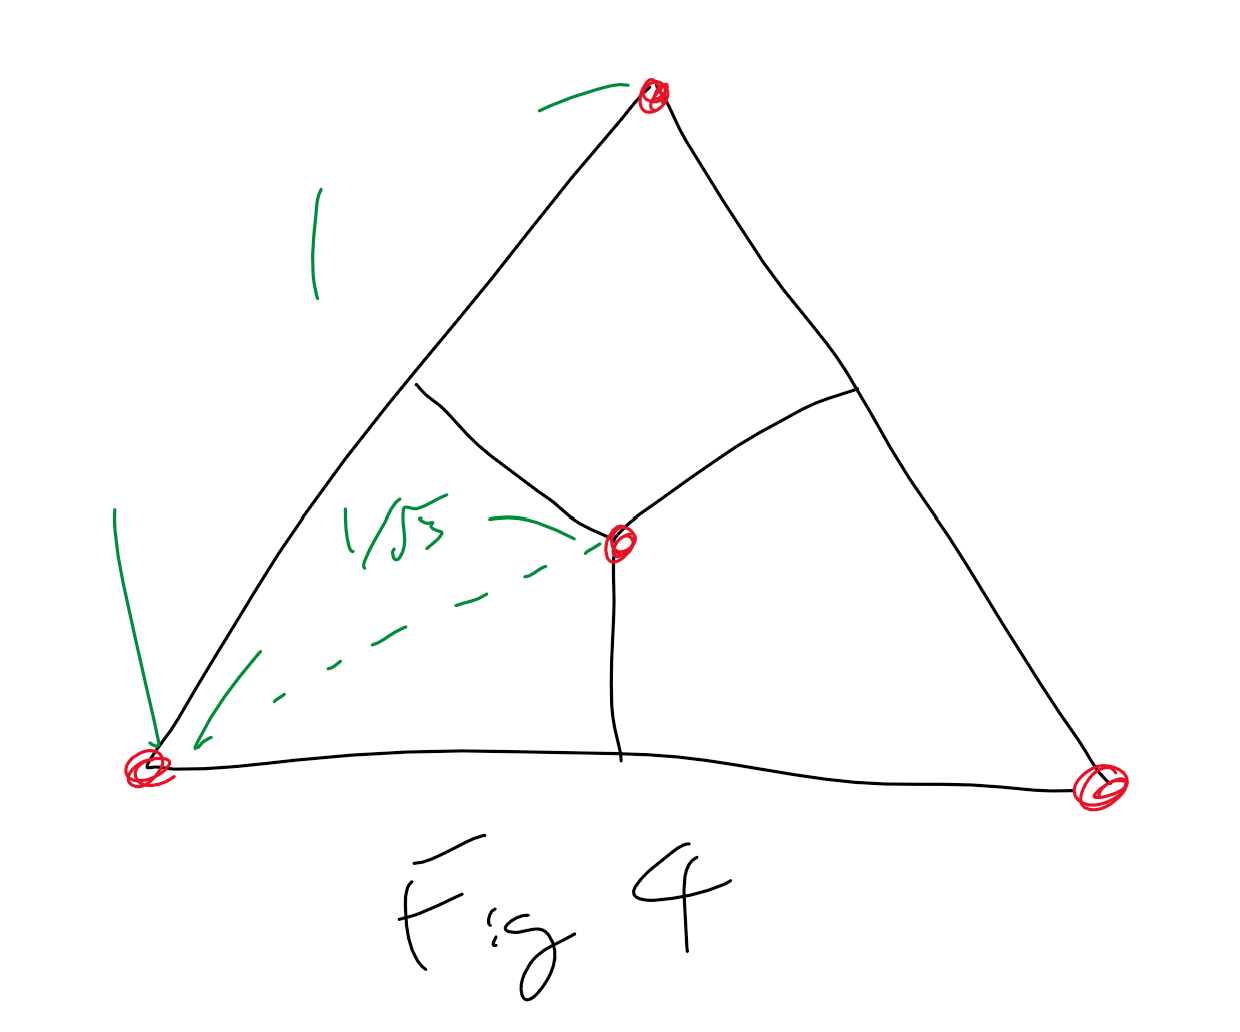
\includegraphics[width = .225\linewidth]{Figure2.png}
 \end{center}
Consider the slicing of the triangle demonstrated in figure 4. 
Each of the three covers have a diameter of $1/\sqrt{3}$. By the 
pigeonhole principle, some two points must fall into the same 
cover. By the definition of diameters, the two points must be 
at most $1/\sqrt{3}$ which shows that there must exist two 
points at least this distance apart. Figrure 4 also demonstrates 
a case that satisfies this upper bound. 
\hfill \qed

\end{document}